\documentclass[11pt,a4paper]{article}
\usepackage{fontspec}
\setmainfont{Times New Roman}
\setsansfont{Arial}
\setmonofont{Menlo}[Scale=.78]
\usepackage[russian,english]{babel}
\usepackage[margin=22mm,headheight=14pt]{geometry}
\usepackage{amsmath,booktabs,array,tabularx,graphicx}
\usepackage{unicode-math}
\setmathfont{texgyretermes-math.otf}
% keep justification stretch out of the spaces around = and + in inline formulas
\thickmuskip=5mu plus 1mu
\medmuskip=4mu plus 1mu minus 2mu
\usepackage{microtype,xcolor,hyperref,natbib,enumitem,caption,fancyhdr,placeins,needspace}

\definecolor{ink}{HTML}{182636}
\definecolor{blue}{HTML}{315A87}
\definecolor{green}{HTML}{16806A}
\definecolor{pale}{HTML}{EDF3F8}
\definecolor{mint}{HTML}{EAF5F1}
\definecolor{warm}{HTML}{F7F2E9}
\definecolor{gray}{HTML}{758190}
\hypersetup{colorlinks=true,linkcolor=blue,citecolor=blue,urlcolor=blue}
\captionsetup{font=small,labelfont={bf,color=ink},skip=5pt}
\setlist{nosep,leftmargin=*}
\setlength{\emergencystretch}{3em}
\setlength{\parskip}{2pt}
\setlength{\parindent}{1.25em}
\pagestyle{fancy}
\fancyhf{}
\fancyhead[L]{\small\color{gray} Событийная память с адресуемыми источниками}
\fancyfoot[C]{\color{gray}\thepage}
\renewcommand{\headrulewidth}{.25pt}

\newcommand{\raw}{RAW}
\newcommand{\events}{EVENTS}
\newcommand{\episodes}{EPISODES}
\newcommand{\pp}{\,\text{п.п.}}
\newcommand{\method}{\textsc{Elem}}
\newcommand{\resultbox}[1]{%
  \begin{center}\setlength{\fboxsep}{9pt}%
  \colorbox{mint}{\parbox{.93\linewidth}{#1}}\end{center}}
\newcommand{\warningbox}[1]{%
  \begin{center}\setlength{\fboxsep}{9pt}%
  \colorbox{warm}{\parbox{.93\linewidth}{#1}}\end{center}}

\begin{document}
\selectlanguage{russian}
\thispagestyle{empty}
\begin{center}
{\sffamily\bfseries\fontsize{15.5}{19.22}\selectfont
Событийная память с адресуемыми источниками\par}
\vspace{3.4mm}
{\sffamily\color{gray}\fontsize{11}{14}\selectfont
Доставка свидетельств, темпоральные вопросы\\ и границы переноса в многосторонних диалогах\par}
\vspace{5mm}
{\color{gray}\rule{.16\linewidth}{.4pt}}
\vspace{4mm}

{\sffamily\fontsize{10.8}{13}\selectfont Ярослав Лихачев\par}
\vspace{1.2mm}
{\sffamily\color{gray}\fontsize{9.4}{12}\selectfont Независимый исследователь\par}
\vspace{1.2mm}
{\sffamily\color{gray}\fontsize{9}{11}\selectfont 17 сентября 2026\par}
\end{center}
\vspace{-3mm}

\begin{abstract}
Как сделать изменяющиеся факты длинного группового разговора доступными для
поиска, не теряя их первоисточник? Мы предлагаем событийную память с
адресуемыми источниками (\method): каждое событие несёт самостоятельное
поисковое описание, владельца точки зрения, субъект, время и неизменяемые пары
\emph{source ID + дословная цитата}. Память строится до чтения вопросов, события
ранжируются вместе с исходными сообщениями, а найденное событие раскрывается
обратно в первичные реплики.

Событийный индекс улучшает доставку размеченных свидетельств относительно
сильного dense RAW. На 2400 вопросах EverMemBench он повышает precision
gold-источников на $3{,}21\pp$ (95\% ДИ $[2{,}84;3{,}59]$) и recall на
$0{,}64\pp$ ($[0{,}48;0{,}80]$), возвращая в среднем меньше уникальных источников
(9,47 против 10,00) и больше gold-попаданий (2,245 против 2,129). Направление
сохраняется в каждом из пяти проектов, а на SocialMemBench, с памятью более
раннего экстрактора, рост precision сохраняется при пересэмплировании
разговорных сетей.

На exploratory-срезе Temporal Duration ($n=300$) события достигают 19,3\%
accuracy против 14,0\% у RAW и у HyDE при приближённо равном токен-бюджете и
одинаковом хронологическом порядке: преимущество сохраняется после контролей
объёма, порядка и расширения запроса. Срез выбран post hoc, и с поправкой на
выбор категории сигнал не достигает подтверждающего статуса.

Полная система достигает 47,16\% macro accuracy в adapter evaluation
EverMemBench, выше опубликованных memory-систем с тем же answer model в
описательном сравнении; собственный RAW получает 46,34\%. В парных сравнениях
средний прирост accuracy от событий и добавочный прирост от связывания в
эпизоды не установлены, перенос между бенчмарками неоднороден. Работа
показывает, что доставку источников и качество ответа нужно оценивать
раздельно: событийный слой устойчиво улучшает первое, а связь со вторым
остаётся открытым вопросом.
\end{abstract}

\section{Введение}

Разговорная память сталкивается с конфликтом двух целей. Для поиска удобно
хранить самодостаточное описание: «Алексей сообщил, что больше не придёт на встречу».
Для проверки нужен исходный материал: кто именно это написал, когда и какими
словами. Если заменить историю summary, ответ становится доступнее, но исчезает
граница между свидетельством и интерпретацией. Если хранить только сообщения,
сохраняется доказательство, но поздний вопрос должен заново угадать все
эллиптические, разнесённые и изменившиеся реплики.

Эта проблема особенно заметна в группе. Автор сообщения, владелец мнения и
субъект высказывания могут быть тремя разными людьми. Одновременно идут
несколько тем, а позиционная близость в потоке не означает принадлежность к
одной линии разговора. Наконец, состояния эволюционируют: «буду на встрече»
через неделю сменяется «уезжаю; на встречу не приду». Плоский профиль легко либо сохранит
обе версии как действующие, либо сотрёт первую и лишит систему возможности
объяснить изменение.

\begin{figure}[ht]
\centering
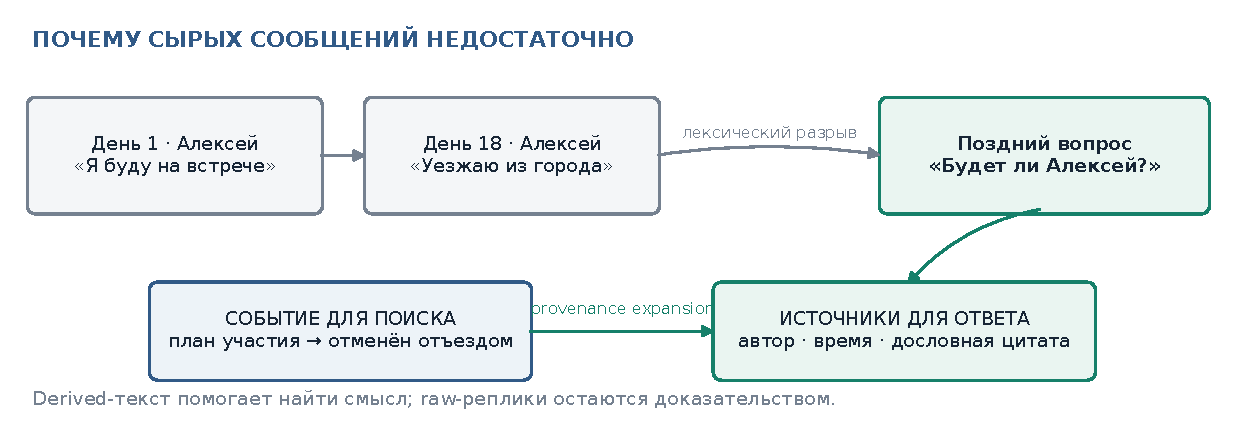
\includegraphics[width=\linewidth]{figures/concept.pdf}
\caption{Двухпредставная память: нормализованное событие служит семантическим
мостом, а ответ строится с возвращёнными первичными репликами. Пример
иллюстративный и не входит в бенчмарк.}
\label{fig:concept}
\end{figure}

Мы предлагаем рассматривать derived memory не как новый источник истины, а как
\emph{индекс над свидетельствами}. В нашей реализации, \method{}, событие
содержит (i) текст, оптимизированный для semantic retrieval; (ii) тип,
владельца точки зрения, субъект и наблюдаемое время; (iii) неизменяемый набор
source IDs и буквальных цитат. События конкурируют с raw turns в одном
векторном top-$k$, а выбранные derived-документы раскрываются обратно в
сообщения. Эпизоды~--- опциональная надстройка: они связывают пересмотр,
подтверждение и дополнение, но не заменяют события и их источники.

Центральный вопрос работы: \emph{помогает ли событийный индекс находить
свидетельства, распределённые между участниками, сообщениями и моментами
времени, сохраняя доступ к первоисточникам?} Вопросы о длительности и смене
состояния~--- трудный частный случай этой задачи. Мы отвечаем в три шага:
измеряем доставку размеченных источников на всех вопросах, проверяем
temporal-преимущество контролями объёма, порядка и расширения запроса и
определяем, что добавляют связывание в эпизоды и перенос на другие бенчмарки.

\paragraph{Вклады.}
\begin{enumerate}
\item \textbf{Метод.} Событийный индекс с адресуемыми источниками: поисковое
описание отделено от неизменяемой опоры, событие несёт владельца точки зрения,
субъект, время и пары \emph{source ID + дословная цитата}, а найденное событие
раскрывается обратно в исходные сообщения.
\item \textbf{Улучшение доставки свидетельств.} На всех 2400 вопросах
EverMemBench событийный индекс повышает precision и recall доставленных
gold-источников относительно сильного dense RAW, возвращая меньше уникальных
источников и больше gold-попаданий; направление сохраняется во всех пяти проектах
и поддерживается на SocialMemBench.
\item \textbf{Раздельная оценка доставки и ответа.} Полная система достигает
47,16\% macro accuracy в adapter evaluation EverMemBench; temporal-преимущество
событий сохраняется после контролей бюджета, порядка и HyDE; парные сравнения
определяют границы пользы: средний прирост accuracy от событий и от связывания в
эпизоды не установлен, перенос между тремя бенчмарками неоднороден.
\end{enumerate}
Память, прогоны и статистика запечатаны, а числа статьи пересчитываются офлайн
(приложение~\ref{app:reproduce}).

\section{Связанные работы}

\paragraph{Память агентов и разговорные задачи.}
Generative Agents соединяют поток опыта, retrieval и рефлексию \citep{park2023};
MemGPT управляет уровнями контекста \citep{packer2023}. Mem0 консолидирует
факты \citep{chhikara2025mem0}, Zep/Graphiti использует временной граф
\citep{rasmussen2025zep}, A-MEM связывает заметки \citep{xu2025amem},
Hindsight разделяет факты, опыт и beliefs \citep{latimer2025hindsight},
HippoRAG реализует графовую ассоциацию \citep{gutierrez2024hipporag}.
В отличие от универсального memory manager, наша оценка сосредоточена на
многостороннем разговоре со стабильными идентификаторами участников.
LoCoMo и LongMemEval исследуют многосессионную память \citep{maharana2024,wu2024};
EverMemBench, GroupMemBench и SocialMemBench добавляют соответственно длинные
совместные проекты, reply-структуру и социальную атрибуцию
\citep{hu2026,yang2026,owolabi2026}.

\paragraph{Ближайшие представления для поиска.}
Dense X Retrieval индексирует атомарные самостоятельные пропозиции
\citep{chen2023densex}. RAPTOR строит иерархию summary; в collapsed-tree
режиме исходные листья и производные узлы ранжируются совместно
\citep{sarthi2024raptor}. Самостоятельные утверждения и совместный пул raw и
derived документов, таким образом, известны. \method{} переносит их на
меняющиеся разговорные состояния: событие явно разделяет автора, владельца
мнения и субъекта, несёт наблюдаемое время и пофактовую пару \emph{source ID +
дословная цитата}, а адрес источника не зависит от поискового описания и версии
эпизода. Экспериментально мы сравниваем эту конструкцию с собственным сильным
RAW и разделяем вклад доставки источников, объёма контекста, порядка и episode
linking; прямого сравнения с proposition retrieval или summary с той же
provenance в работе нет (§\ref{sec:limits}).

\paragraph{Расширение запроса и проверяемость.}
HyDE генерирует гипотетический документ для embedding запроса
\citep{gao2023hyde}; событийная память нормализует корпус заранее.
Мы сравниваем их на Temporal Duration с выравниванием бюджета и порядка.
Как и работы по RAG и цитированию \citep{lewis2020,gao2023}, мы отделяем
поиск опоры от качества ответа: существующий указатель не доказывает
семантическую корректность пересказа.

\section{Формулировка задачи}
\label{sec:problem}

Пусть $M=(m_1,\ldots,m_n)$~--- история одного bounded conversation space.
Сообщение $m_i=(id_i,g_i,a_i,t_i,x_i)$ содержит пространство, автора, время и
текст. Построитель $B$ получает только $M$ и создаёт память $\mathcal{D}$ до
открытия QA. Для запроса $q$ retrieval выбирает документы $R_k(q,\mathcal{D})$,
после чего генератор отвечает по раскрытому контексту $C_q$.

Мы различаем три свойства:
\begin{enumerate}
\item \textbf{целостность указателя}: source ID существует, а цитата буквально
содержится в нём;
\item \textbf{семантическая поддержка}: текст источника действительно влечёт
derived-описание;
\item \textbf{правильность ответа}: генератор верно использовал доставленный
контекст.
\end{enumerate}
Механическая проверка гарантирует только первое. Второе требует entailment- или
human-аудита, третье измеряется benchmark scoring.

\section{Метод}
\label{sec:method}

\subsection{Неизменяемое событие}

Событие имеет вид
\[
e=(z,o,s,k,r,\tau,P,L),
\]
где $z$~--- самодостаточный index text, $o$~--- владелец точки зрения, $s$~---
субъект, $k$~--- тип события, $r$~--- temporal mode, $\tau$~--- наблюдаемое
время, $P$~--- evidence, $L$~--- локальный контекст. Evidence состоит из пар
$(id_i, quote_i)$; время выводится из реальных timestamps источников.

Разделение $o$ и $s$ позволяет представить «А назвал Б ненадёжным» как мнение
А о Б, а не как безусловный факт о Б; корректность этих полей определяется
качеством извлечения. Типы
охватывают состояние, мнение, решение, обязательство, отношение, исключение и
категорию \texttt{other}. Разговорная реакция без долговременного содержания может не
порождать события; действует cap не более двух событий на один turn.

\needspace{16\baselineskip}
\paragraph{Пример.}
Иллюстративный фрагмент одной рабочей сессии, не из бенчмарка:
\begin{quote}\small
10:02, Марина: «Релиз двигаем на пятницу~--- у Олега не закрыт платёжный модуль».\\
10:05, Олег: «Сделаю до вечера».\\
18:40, Олег: «Готово, можно катить».
\end{quote}
Через неделю задан вопрос: «Кто задерживал релиз и закрыл ли он свою часть?»
Ответ содержится в реплике 18:40, но в ней нет ни релиза, ни платёжного модуля,
ни имени того, о ком идёт речь: связь с вопросом существует только через
соседние сообщения. Схема допускает два события:
\begin{itemize}
\item $e_1$: $z$~= «Марина связала перенос релиза на пятницу с незакрытым
платёжным модулем Олега»; $o$~= Марина, $s$~= Олег, $\tau$~= 10:02;
$P$: (10:02, «у Олега не закрыт платёжный модуль»).
\item $e_2$: $z$~= «Олег сообщил, что закрыл платёжный модуль»; $o$~= Олег,
$s$~= платёжный модуль, $\tau$~= 18:40; $P$: (18:40, «Готово, можно катить»);
сообщения 10:02 и 10:05 входят в $L$ как контекст, разрешающий «готово».
\end{itemize}
Индексный текст $e_2$ делает короткое подтверждение доступным поиску по словам
вопроса, а цитата указывает на исходную реплику. Здесь же видна граница этой
гарантии. Цитата подтверждает, что реплика существует и написана Олегом в 18:40,
но не подтверждает интерпретацию «закрыл платёжный модуль»: она опирается на
сообщения из $L$. Генератору вместе с событием возвращаются только источники из
$P$; сообщения из $L$ попадают в контекст, лишь если их независимо находит
поиск. Поэтому поясняющую реплику 10:02 лучше включать в $P$, а проверка
буквальности цитат этого не обеспечивает: это семантическая поддержка
(свойство~2 в §\ref{sec:problem}), а не целостность указателя. Поля выполняют
разные роли: $o$ отличает утверждение Марины \emph{об} Олеге от собственного
сообщения Олега, $s$ задаёт, о ком или о чём факт, а $\tau$ отделяет состояние
«не закрыт» от более позднего «закрыт». Пример иллюстрирует роль полей схемы;
измеренные эффекты приведены в §\ref{sec:delivery}--\ref{sec:episodes}.

\subsection{Query-independent extraction и валидация}

История разделяется по benchmark-сессиям: в
EverMemBench~--- день и группа; в GroupMemBench~--- канал/фаза с блоками до 40
сообщений. Forced structured output допускает пустой список. Затем
детерминированный валидатор удаляет выдуманные IDs, отсутствующие цитаты,
content-free значения и некорректные enum. Локальный context может помочь
разрешить местоимение, но не становится evidence автоматически.

\subsection{Опциональные версионные эпизоды}

Эпизод $E_j=((e_1,\rho_1),\ldots,(e_t,\rho_t))$~--- append-only линия, где
$\rho\in\{\texttt{create},\texttt{revise},\texttt{reaffirm},\texttt{augment}\}$.
Для нового события кандидаты ищутся только внутри conversation network.
Скор равен
\[
S(e,E)=0{,}6\cos(\phi(z_e),\phi(A_E))+0{,}4\cos(\phi(z_e),\phi(z_{last(E)})).
\]
Здесь $A_E$~--- конкатенация последних пяти событий, $z_{last(E)}$~---
последнее событие; $\phi$~--- локальный MiniLM embedding для linking.
Три лучших эпизода поступают LLM-resolver. При пустом пуле, невалидном выборе
или confidence ниже 0,5 создаётся новый episode; это защитная ветвь, а не
дополнительный поиск. Для retrieval ответов используется отдельный embedding
benchmark adapter. Для индекса хранится hot-view последних пяти событий,
но cold events и evidence не удаляются. Мы предполагаем, что false split обходится
дешевле false merge: разделённые события всё ещё могут независимо попасть в
retrieval, тогда как ошибочное слияние может приносить посторонние источники в
последующие обращения; частоты обеих ошибок не измерялись.

\subsection{Единый поиск и provenance expansion}

Raw turn и derived document имеют общий интерфейс
\[
d=(id,\ kind,\ index\_text,\ render\_text,\ source\_ids).
\]
Вектор вопроса
сравнивается с одним пулом; top-$10$ может содержать оба типа. После ranking
каждый event/episode раскрывается в уникальные raw turns. Генератор видит
derived-текст как навигационную подсказку и датированные speaker-grounded
источники как основание ответа.

Derived memory проходит тот же критерий релевантности, что и raw history;
статические пользовательские профили не добавляются.

\FloatBarrier
\begin{figure}[t]
\centering
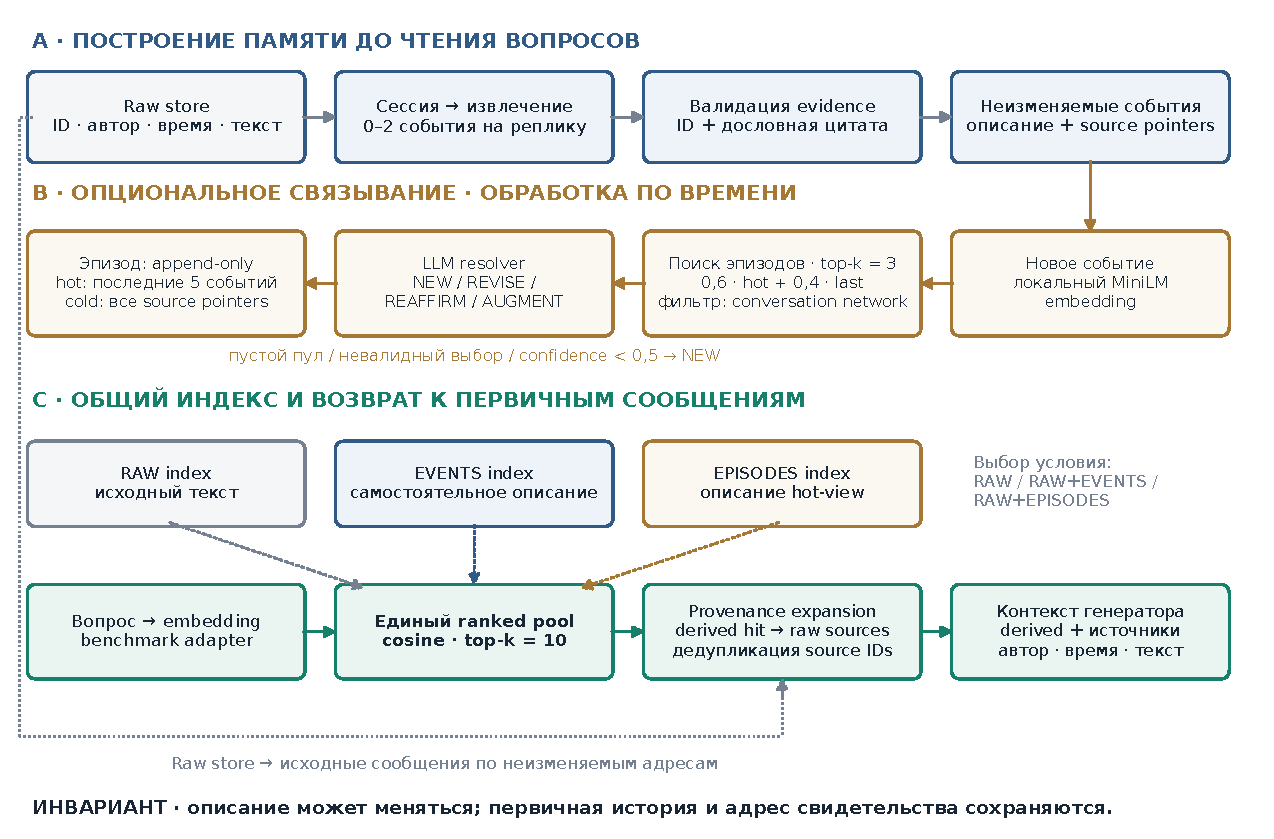
\includegraphics[width=\linewidth]{figures/architecture.pdf}
\caption{Полная архитектура. Память строится query-independently и запечатывается
до QA. В основном варианте raw turns и episodes ранжируются совместно; в
абляции episodes заменяются отдельными events. Derived-hit всегда раскрывается
в raw sources.}
\label{fig:architecture}
\end{figure}

\section{Экспериментальный протокол}

\subsection{Данные и условия}

\begin{table}[ht]
\centering\small
\begin{tabularx}{\linewidth}{lrrX}
\toprule
Benchmark & QA & пространства & Основная проверка\\
\midrule
EverMemBench & 2400 & 5 проектов & 9 типов задач; temporal controls\\
SocialMemBench & 1031 & 43 сети & социальная атрибуция, нормы, updates\\
GroupMemBench & 745 & 4 домена & reply structure, implicit, multi-hop\\
\bottomrule
\end{tabularx}
\caption{Использованные внешние наборы. Для GroupMemBench 102 первоначально
пустых generation outputs восстановлены отдельным запечатанным amendment;
исходный protocol result сохранён.}
\label{tab:data}
\end{table}

Основной paired baseline~--- сильный dense \raw{}, а не слабый keyword-only
поиск. Условия \events{} и \episodes{} добавляют производные документы в тот же
top-$10$. Для Temporal Duration дополнительно контролируются токен-бюджет и
хронологический порядок; в контролях перестановки множество источников
фиксировано внутри каждого условия, но не между RAW и EVENTS. HyDE генерирует
гипотетический документ только для embedding запроса и возвращает те же raw
documents. Все варианты
используют одинаковые official answer/judge prompts внутри соответствующего
benchmark adapter.

EverMemBench использует GPT-4.1-mini для ответа, Gemini-3-Flash-preview для
open-answer judge, text-embedding-3-large для retrieval и
gpt-4o-mini-2024-07-18 для построения памяти. Answer- и judge-модели, их промпты
и точное скорирование multiple choice взяты из официального harness; провайдеры
запинены (OpenAI и Google AI Studio соответственно) с отключёнными fallback~---
это согласует модели оценки, но не все остальные компоненты чужих систем. Ответы и judge EverMemBench
используют \texttt{temperature}${}=0$. SocialMemBench следует
GPT-4o-mini official-compatible harness. GroupMemBench использует GPT-5
официального прогона; версия модели у провайдера не была запинена датой, поэтому
побайтовое воспроизведение этих чисел не гарантировано. Сравнения между бенчмарками не интерпретируются как
сравнение моделей.

\subsection{Метрики и статистика}
\label{sec:stats}

Мы сообщаем micro accuracy, macro по официальным типам вопросов и парные
разницы условий. Для вопроса $q$ пусть $U_q$~--- множество уникальных
раскрытых источников, $G_q$~--- gold anchors, опубликованные бенчмарком:
\[
P_q=\frac{|U_q\cap G_q|}{|U_q|},\qquad
R_q=\frac{|U_q\cap G_q|}{|G_q|}.
\]
При пустом $U_q$ precision равна нулю, при пустом $G_q$ recall по scorer равна
единице; в проверенных Ever-вопросах $G_q$ непусто. В таблицах приведены
\emph{средние по вопросам отношения}, а не отношение суммарных попаданий
к суммарному числу источников. Эти метрики измеряют доставку размеченной опоры,
не entailment, достаточность контекста или правильность пользовательских цитат.

95\% ДИ для Ever и Group получены парным question bootstrap; для переноса на
Social дополнительно пересэмплируются 43 разговорные сети. Accuracy
сравнивается exact McNemar. Question-level интервалы описывают исследованный
набор: его вопросы не равнозначны независимым проектам. Поэтому для evidence
мы также показываем эффект по каждому Ever-проекту и leave-one-project-out
чувствительность (приложение~\ref{app:verification}).

Temporal Duration выбран после просмотра полного разреза, поэтому его анализ
обозначен как exploratory; поправка на выбор категории приведена в
§\ref{sec:temporal}. Протоколы, revisions и запечатывание артефактов вынесены в
приложение.

\section{Результаты: уровень системы и парные сравнения}

Здесь разделены два вопроса. Насколько сильна полная система в абсолютном
выражении, показывает описательное сравнение с опубликованными строками
(§\ref{sec:external}). Что добавляет именно событийная память, показывают только
парные сравнения с нашим RAW на тех же вопросах (§\ref{sec:paired}) и контроли
§\ref{sec:mech}. Первый ответ характеризует достигнутый уровень системы, второй~---
вклад событийного слоя.

\subsection{Сравнение с опубликованными системами}
\label{sec:external}

\paragraph{EverMemBench.}
\begin{figure}[t]
\centering
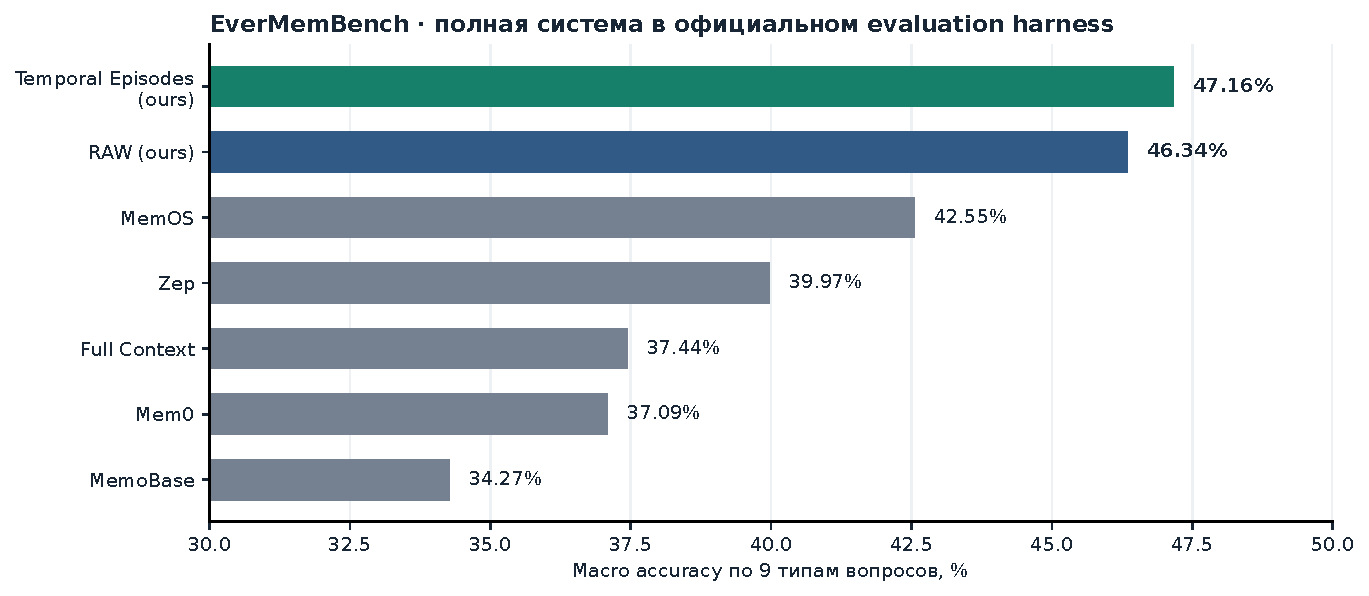
\includegraphics[width=.96\linewidth]{figures/ever_leaderboard.pdf}
\caption{Macro accuracy на девяти категориях EverMemBench с answer-backbone
GPT-4.1-mini. Опубликованные результаты взяты из benchmark paper
\citep{hu2026}; наши строки получены adapter evaluation поверх официального
harness. Сравнение описательное: не официальный leaderboard submission и не
парный тест против чужих систем.}
\label{fig:leaderboard}
\end{figure}

Полная система \episodes{} достигает \textbf{47,16\% macro}, а \raw{}~---
46,34\%. Наш adapter result выше значений, reported \citet{hu2026} с тем же
answer-backbone: MemOS 42,55\%,
Zep 39,97\%, Mem0 37,09\%, Full Context 37,44\% и MemoBase 34,27\%.
Разница с лучшей опубликованной memory-системой составляет 4,61 п.п.

\begin{table}[ht]
\centering\small
\begin{tabular}{@{}lrrrrr@{}}
\toprule
Система & Macro & Multi-hop & Temporal & Update & Style\\
\midrule
\episodes{} (ours) & 47,16 & 13,25 & 20,00 & 47,39 & 38,07\\
\events{} (ours) & 46,82 & 13,25 & 16,33 & 47,01 & 33,52\\
\raw{} (ours) & 46,34 & 12,85 & 12,33 & 46,27 & 30,11\\
\midrule
MemOS & 42,55 & 18,88 & 15,67 & 45,15 & 28,98\\
Zep & 39,97 & 8,03 & 13,00 & 43,66 & 26,70\\
Mem0 & 37,09 & 11,24 & 6,33 & 51,87 & 22,73\\
MemoBase & 34,27 & 12,85 & 18,00 & 30,60 & 17,05\\
\bottomrule
\end{tabular}
\caption{Абсолютный уровень EverMemBench, accuracy в процентах; answer model
GPT-4.1-mini. Чужие строки: таблица 4 в arXiv:2602.01313v3
\citep{hu2026}; наши строки: полные прогоны без token/order controls.
Macro усредняет все девять типов, остальные столбцы показывают четыре
диагностических среза. Между блоками нет парного статистического теста.}
\label{tab:ever-external}
\end{table}

На Temporal наш \episodes{} получает 20,00\% при 6,33--18,00\% у
опубликованных memory rows. Профиль по категориям неоднороден: MemOS выше на
Multi-hop, Mem0~--- на Update.

Сравнение фиксирует достигнутый уровень полного adapter; чужие системы не
перезапускались на одной инфраструктуре. Сильный собственный \raw{} (46,34\%)
показывает, что большую часть этого уровня обеспечивают retrieval и answer
model, а добавочный вклад памяти измеряется парно в §\ref{sec:paired}.

\paragraph{SocialMemBench.}
На SocialMemBench полная система достигает MeanQ .368 (\episodes{}) и .358
(\raw{}): практически на уровне опубликованного full-context .369 и выше
перечисленных benchmark memory rows (лучший Subject-Mem .321).

\begin{table}[ht]
\centering\small
\begin{tabular}{@{}lrrrrr@{}}
\toprule
Система & MeanQ & Атрибуция & Решения & ToM & Смена состояния\\
\midrule
\episodes{} (ours) & .368 & .863 & .691 & .262 & .259\\
\raw{} (ours) & .358 & .825 & .716 & .251 & .233\\
\midrule
Subject-Mem & .321 & .780 & .610 & .240 & .220\\
SMG & .213 & .440 & .690 & .110 & .100\\
Graphiti & .178 & .460 & .610 & .050 & .070\\
LangMem & .162 & .390 & .560 & .060 & .090\\
Mem0 & .143 & .310 & .570 & .050 & .070\\
Cognee & .120 & .250 & .590 & .100 & .010\\
\bottomrule
\end{tabular}
\caption{SocialMemBench: question-weighted scores (0--1), не binary accuracy.
Все строки используют GPT-4o-mini. Чужие результаты: таблица 4
\citep{owolabi2026}; наши: frozen official-v1 harness.
Столбцы соответствуют Q4/AP, Q2/GD, Q5/TM и Q8/TS.
Сравнение с внешними строками описательное.}
\label{tab:social-external}
\end{table}

Сравнение показывает разные требования к памяти: adapter получает высокую
атрибуцию (.863 у \episodes{}), а theory-of-mind и восстановление смены состояния
остаются трудными даже при сохранённых источниках. На групповых решениях
\episodes{} уступают нашему \raw{} (.691 против .716), поэтому высокий общий уровень
отражает весь adapter, а не только linking.

\paragraph{GroupMemBench.}
У GroupMemBench внешние результаты также зависят от типа задачи
(приложение~\ref{app:group-external}). Например, опубликованный Hindsight
достигает 54,94\% на Temporal, но 17,76\% на Update; наш EPISODES~---
36,42\% и 23,36\% соответственно. При этом опубликованный BM25 достигает
54,94\% на Temporal и 25,23\% на Update: сравнение только с тяжёлыми
memory-системами скрыло бы сильную простую альтернативу.

\subsection{Парные сравнения внутри наших условий}
\label{sec:paired}

\paragraph{EverMemBench.}
\begin{table}[ht]
\centering\small
\begin{tabular}{lrrrr}
\toprule
Условие & Micro & Macro & Evid. recall & Evid. precision\\
\midrule
\raw{} & 49,46 & 46,34 & 8,08 & 21,29\\
\events{} & 49,83 & 46,82 & 8,71 & \textbf{24,50}\\
\episodes{} & \textbf{50,21} & \textbf{47,16} & \textbf{10,75} & 22,45\\
\bottomrule
\end{tabular}
\caption{EverMemBench, все 2400 QA, проценты. Macro~--- среднее по девяти
официальным типам вопросов; micro~--- по отдельным QA.}
\label{tab:ever-main}
\end{table}

На micro уровне \episodes{} улучшают 49,46\%$\rightarrow$50,21\%:
$+0{,}75\pp$, 95\% ДИ $[-0{,}5;+2{,}0]$, $p=.256$. \events{} дают 49,83\%:
$+0{,}38\pp$, ДИ $[-0{,}8;+1{,}6]$, $p=.589$. Оба интервала включают ноль: средний
прирост accuracy в парном сравнении не установлен.

\paragraph{Перенос между бенчмарками.}
\begin{figure}[ht]
\centering
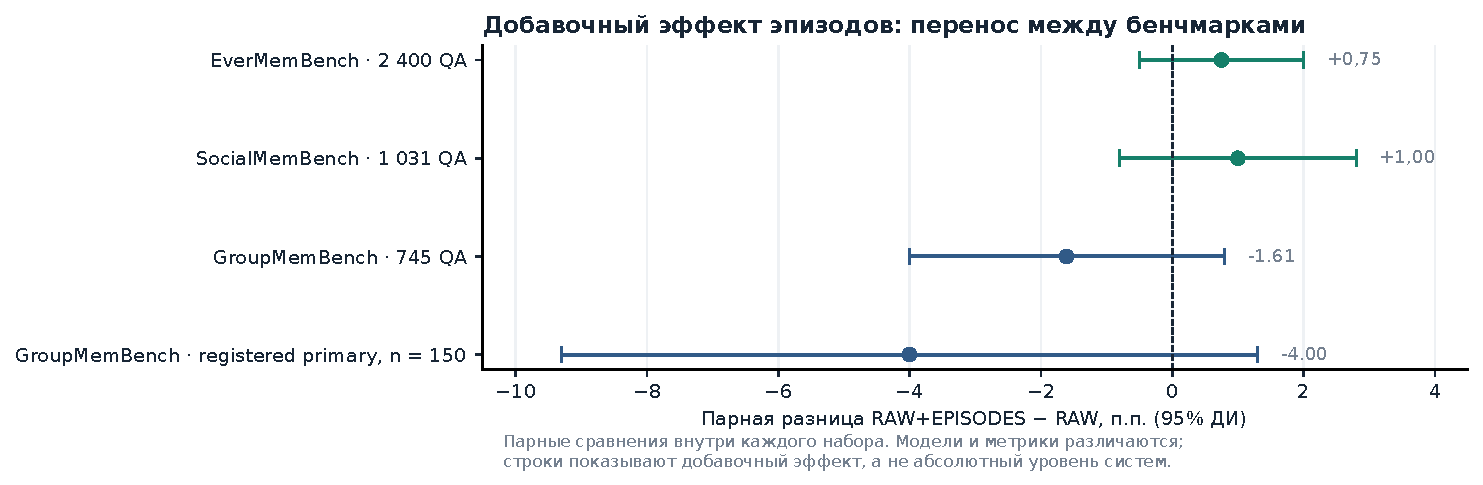
\includegraphics[width=.92\linewidth]{figures/transfer.pdf}
\caption{Парные разницы \episodes{}$-$\raw{} внутри каждого набора с question-
или network-bootstrap 95\% ДИ. Показаны только парные разницы: метрика (accuracy
против MeanQ), протоколы и answer-модели у трёх наборов различаются. Group приведён после
targeted repair пустых генераций; его отдельно зарегистрированный
temporal/update endpoint ($n=150$ из 745) показан отдельной строкой. Ни один
интервал не исключает ноль.}
\label{fig:transfer}
\end{figure}

На SocialMemBench парная разница \episodes{}$-$\raw{} составляет $+0{,}010$ MeanQ,
network-bootstrap 95\% ДИ $[-.008;+.028]$: средний выигрыш в MeanQ не установлен.

На уровне доставки Social поддерживает направление EverMemBench. Precision
доставленных источников растёт относительно \raw{} у flat-памяти ($+0{,}90\pp$,
network-bootstrap 95\% ДИ $[+0{,}66;+1{,}19]$), versioned ($+0{,}86\pp$,
$[+0{,}61;+1{,}16]$) и episodes ($+0{,}34\pp$, $[+0{,}15;+0{,}54]$); все три
интервала исключают ноль. Результат получен на другой структуре разговоров и с
другой answer model. Схемы памяти не идентичны: flat и versioned построены более
ранним экстрактором, а базовый evidence recall Social (67,5\%) существенно выше,
чем у Ever, поэтому абсолютные величины эффектов между наборами не сопоставимы.

На GroupMemBench перенос неоднороден. На заранее зарегистрированном Group primary
(Finance+Technology, knowledge update+temporal, $n=150$) после восстановления
пустых ответов \raw{} достигает 37,3\%, \episodes{}~--- 33,3\%:
$\Delta=-4{,}0\pp$, ДИ $[-9{,}3;+1{,}3]$; на всех 745 QA~--- 43,1\% против 41,5\%,
$\Delta=-1{,}6\pp$, ДИ $[-4{,}0;+0{,}8]$. Направление отрицательное и сохраняется
после repair; интервалы включают ноль. Детали 102 восстановленных генераций и
исходного protocol result приведены в приложении~\ref{app:repair}.

\section{Событийное представление: доставка и темпоральные ответы}
\label{sec:mech}

Сначала рассмотрим прямое изменение найденных источников, затем~--- его связь с
качеством ответа. Такой порядок оценивает поисковую надстройку отдельно от общего
уровня answer model.

\subsection{Доставка свидетельств: основной результат}
\label{sec:delivery}

Мы сравниваем парно, по каждому вопросу, долю доставленных gold-источников
(recall) и их плотность в контексте (precision) на всех 2400 вопросах, без отбора
среза.

\begin{figure}[t]
\centering
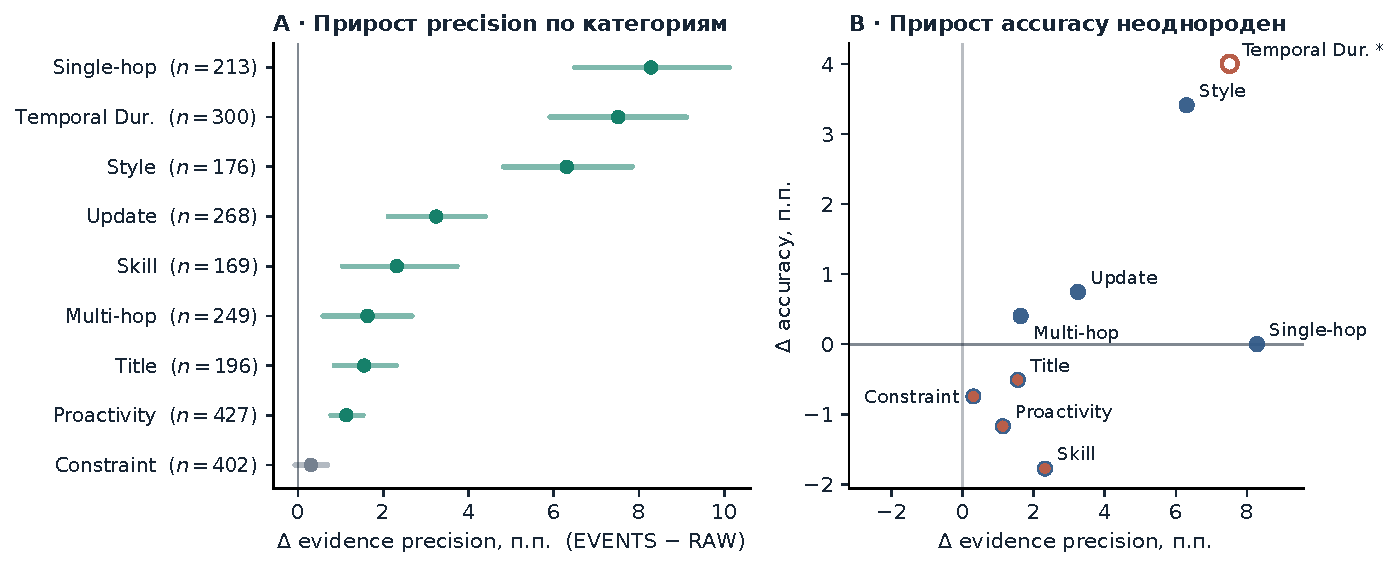
\includegraphics[width=\linewidth]{figures/dissociation.pdf}
\caption{Доставка свидетельств и accuracy. \textbf{A}: парная разница evidence precision
\events{}$-$\raw{} по девяти официальным категориям, все 2400 вопросов,
question bootstrap 95\% ДИ; знак положителен везде, интервал включает ноль
только у Constraint. \textbf{B}: та же ось против сдвига accuracy; звёздочкой
отмечен post hoc discovery-срез. Категория с наибольшим приростом доставки
(Single-hop, $+8{,}28\pp$) стоит у потолка accuracy 89,7\% и не выигрывает ничего.
Точки описывают неоднородность категорий, а не причинную связь доставки и ответа.}


\label{fig:dissociation}
\end{figure}

\begin{table}[ht]
\centering\small
\begin{tabular}{lrrr}
\toprule
Условие & Источников & Gold-попаданий & Evid. precision\\
\midrule
\raw{}      & 10,00 & 2,129 & 21,29\\
\events{}   & \textbf{9,47} & \textbf{2,245} & \textbf{24,50}\\
\episodes{} & 12,38 & 2,795 & 22,45\\
\bottomrule
\end{tabular}
\caption{EverMemBench, все 2400 QA: сколько уникальных источников попало в
контекст, сколько из них оказались gold anchors, и какая доля контекста была
gold. В среднем у \events{} меньше источников и больше gold-попаданий, чем у \raw{}.}
\label{tab:delivery}
\end{table}

\events{}$-$\raw{}, парно: precision $+3{,}21\pp$ (95\% ДИ $[+2{,}84;+3{,}59]$,
855 вопросов лучше против 255 хуже), recall
$+0{,}64\pp$ ($[+0{,}48;+0{,}80]$). Знак прироста precision положителен во всех
девяти официальных категориях, ДИ исключает ноль в восьми из девяти
(таблица~\ref{tab:evid-cats}). Эффект не держится на одном проекте: прирост
положителен в каждом из пяти проектов EverMemBench, а при исключении любого
проекта остаётся в пределах 3,11--3,39\pp{} (приложение~\ref{app:verification}).
Событийный индекс, таким образом, приводит в фиксированный top-10 больше
размеченной опоры.

\paragraph{Рост precision не сводится к уменьшению числа возвращённых источников.}
Precision могла бы вырасти только потому, что источников возвращается меньше.
Данные показывают другое: \events{} возвращают в среднем 9,47 источника против
10,00 у \raw{} и \emph{ни на одном} вопросе не больше, но находят больше
gold-попаданий~--- $2{,}245$ против $2{,}129$ на вопрос, дельта $+0{,}117$ (ДИ
$[+0{,}083;+0{,}151]$); в 449 вопросах gold-попаданий строго больше без
увеличения числа источников. Событийный индекс улучшает отбор опоры, а не
просто укорачивает список. По токенам контекст при этом длиннее: derived-текст
событий даёт в среднем 1177 против 1054 токенов \texttt{o200k\_base} (пересчёт
офлайн по запечатанному retrieval), поэтому роль объёма в temporal-результате
проверяется отдельным токен-контролем (§\ref{sec:temporal}). \episodes{} ведут
себя иначе: они повышают recall вместе с объёмом ($+2{,}68\pp$ recall при $+2{,}4$
источника), а их precision растёт слабее ($+1{,}16\pp$).

\paragraph{Query-side расширение этого не воспроизводит.}
На Temporal Duration при приближённо равном бюджете и одинаковом порядке matched
HyDE получает близкий recall~--- 20,7\% против 19,7\% у \events{} (разница
EVENTS$-$HyDE $-1{,}01\pp$, ДИ $[-2{,}20;+0{,}17]$), но заметно более разреженный
контекст: precision у \events{} выше на $+6{,}68\pp$ (ДИ $[+5{,}06;+8{,}27]$).
Против token-matched \raw{} HyDE повышает precision на $+1{,}18\pp$ и recall на
$+1{,}61\pp$. Расширение запроса и нормализация корпуса дают разный профиль
доставки: при близком recall событийный индекс доставляет более плотную опору.
Доминирование \events{} по обеим координатам не установлено: recall у них немного
ниже, а незначимая разница не означает эквивалентности.

\paragraph{Почему низкий recall совместим с высокой accuracy.}
Gold-разметка Ever содержит медианно 27 источников на вопрос
(межквартильный диапазон 21--37; максимум 96), тогда как RAW возвращает десять.
Это задаёт низкую полноту относительно всего reference set.
В RAW 316 из 2400 вопросов получили правильный verdict без единого
доставленного gold anchor; в EVENTS таких вопросов 312.
Gold intersection и accuracy измеряют разные свойства системы; достаточность
свидетельств для ответа отдельно не оценивалась.

\subsection{Temporal Duration: преимущество после контролей}
\label{sec:temporal}

В исходном разрезе Temporal Duration RAW достигает 12,3\%, EPISODES~---
20,0\%. Но эпизоды раскрываются в несколько сообщений: в среднем 17,4
источника против десяти у RAW. Поэтому мы последовательно проверили
расширение raw-контекста, хронологический порядок, отдельные события вместо
linked episodes и HyDE на стороне запроса.

Token matching использует число токенов раскрытого EPISODES-контекста как
целевой бюджет и выбирает ближайший префикс ranked-документов без обрезания
сообщений; это выравнивание бюджета, не побайтовое равенство.
HyDE matched ориентирован на EVENTS-контекст. Chrono-контроли меняют только
порядок уже выбранных блоков, сохраняя их источники.
Средние размеры chrono-контекстов: RAW 2458, EVENTS 2456, HyDE 2451 токен.
Пер-вопросная абсолютная разница EVENTS и RAW имеет медиану 35 токенов
(1,48\%), 95-й перцентиль 97 (4,60\%) и максимум 139 (11,46\%).
Полные отклонения и правила их расчёта приведены в приложении~\ref{app:tokens}.

\begin{figure}[t]
\centering
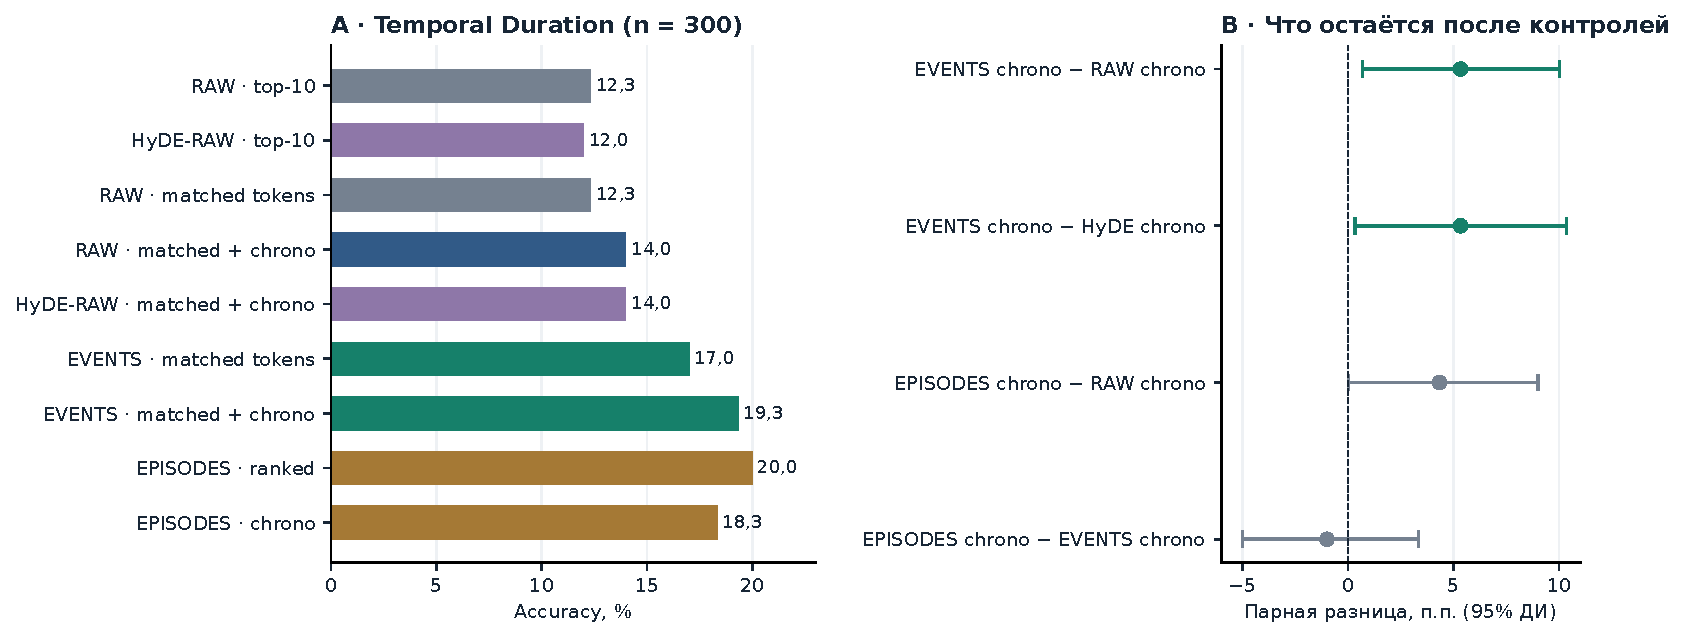
\includegraphics[width=\linewidth]{figures/temporal_controls.pdf}
\caption{Контроли представления, объёма и порядка на exploratory Temporal Duration. EVENTS
chrono сохраняют наблюдаемое преимущество над RAW и HyDE при приближённом
выравнивании токен-бюджета и одинаковом порядке;
EPISODES не превосходят EVENTS. Интервалы~--- question bootstrap 95\%.}
\label{fig:controls}
\end{figure}

\begin{table}[ht]
\centering\small
\begin{tabular}{lrrr}
\toprule
Условие & Accuracy & Evid. recall & Evid. precision\\
\midrule
RAW top-10 & 12,3 & 12,7 & 29,6\\
HyDE-RAW top-10 & 12,0 & 14,1 & 32,4\\
RAW count-matched & 13,3 & 16,6 & 25,1\\
RAW token-matched & 12,3 & 19,1 & 21,5\\
RAW token-matched chrono & 14,0 & 19,1 & 21,5\\
HyDE-RAW token-matched chrono & 14,0 & \textbf{20,7} & 22,6\\
EVENTS token-matched & 17,0 & 19,7 & 29,3\\
EVENTS token-matched chrono & 19,3 & 19,7 & 29,3\\
EPISODES ranked & \textbf{20,0} & \textbf{20,5} & \textbf{31,1}\\
EPISODES chrono & 18,3 & \textbf{20,5} & \textbf{31,1}\\
\bottomrule
\end{tabular}
\caption{Temporal Duration, $n=300$, проценты. Precision и recall~--- средние
пер-вопросных отношений после раскрытия источников.}
\label{tab:controls}
\end{table}

При приближённо равном токен-бюджете и одинаковом порядке \events{} достигают
19,3\% против 14,0\% у \raw{}: $+5{,}33\pp$, 95\% ДИ $[+0{,}67;+10{,}0]$,
номинальное $p=.0402$. Matched HyDE также получает 14,0\%; разница
\events{}$-$HyDE составляет $+5{,}33\pp$, ДИ $[+0{,}33;+10{,}33]$, номинальное
$p=.0479$ (37 выигрышей против 21 проигрыша). Направление положительно во всех
пяти проектах. Вне Temporal Duration, на 2100 вопросах, \events{} дают
$-0{,}14\pp$ (ДИ $[-1{,}33;+1{,}10]$, $p=.877$): преимущество сосредоточено в этом
срезе, а не распределено по всем задачам.

Преимущество сопровождается характерным профилем доставки. События сочетают
recall расширенного RAW (19,7\% против 19,1\%) с precision RAW top-10 (29,3\%
против 29,6\%), тогда как HyDE повышает recall до 20,7\% при precision 22,6\% и
accuracy 14,0\%. Этот профиль согласуется с temporal-преимуществом; связь
доставки и ответа проверяется в §\ref{sec:frontier}.

\paragraph{Статус temporal-сигнала.}
Срез выбран post hoc из девяти категорий. С консервативной Bonferroni-поправкой
номинальные $p=.0402$ и $.0479$ становятся примерно $.36$ и $.43$; при пяти
проектах используемый двусторонний exact sign-flip тест не может достичь
$p<.05$ (минимум $.0625$). Предварительная фиксация matched-HyDE endpoint
охватывает анализ, но не выбор среза. Temporal-результат, таким образом,~---
содержательный exploratory-сигнал, устойчивый к контролям бюджета, порядка и
HyDE, но не подтверждённый эффект.

\subsection{Связь доставки источников с качеством ответа}
\label{sec:frontier}

До расчёта мы записали правило офлайновой проверки: вне Temporal Duration
разделить вопросы по тому, доминируют ли \events{} или \raw{} по recall и precision,
и сравнить направление accuracy. В страте, где \events{} доставляют строго лучшую
опору ($n=650$), accuracy меняется на $+0{,}77\pp$ (ДИ $[-1{,}85;+3{,}54]$); при
доминировании \raw{} ($n=209$)~--- на $-2{,}39\pp$ ($[-6{,}70;+2{,}39]$). Направления
соответствуют гипотезе, но заранее записанный критерий подтверждения не выполнен
(приложение~\ref{app:frontier}).

Этот результат разграничивает установленное и открытое. Улучшение доставки
измеряется непосредственно и устойчиво; его перенос в accuracy на доступных
выборках не подтверждён. Раздельная оценка двух эндпоинтов показывает, какую
пользу событийный слой уже даёт и какую ещё предстоит установить. Проверка
выполнена на ранее изученном наборе, не устанавливает причинного механизма и не
исключает влияния доставки на ответ: интервал в страте с лучшей доставкой
допускает и заметный положительный эффект.

\subsection{Что дают эпизоды сверх событий}
\label{sec:episodes}

В симметричных контролях \episodes{} chrono получают 18,3\%, \events{} chrono~---
19,3\%: разница $-1{,}0\pp$, ДИ $[-5{,}0;+3{,}33]$, $p=.755$. В ранее запечатанном
сравнении ranked episodes (20,0\%) и events chrono (19,3\%) разница составляла
$+0{,}67\pp$, $p=.888$. Добавочный средний выигрыш linking в accuracy не установлен.

Связывание меняет профиль доставки (§\ref{sec:delivery}) и хранит
инспектируемую хронологию пересмотров, подтверждений и дополнений с доступом к
прежним свидетельствам. Для поиска в исследуемом сценарии отдельные события
оказываются более простой основой: разделённые события независимо попадают в
контекст через обычное ранжирование.

\section{Эффективность и инженерные свойства}

\subsection{Стоимость и задержка}

Полный EverMemBench эксперимент зарегистрировал 26\,413 API calls и верхнюю
оценку list-price \$8{,}88. Из них построение памяти gpt-4o-mini стоит \$4,76,
embeddings~--- \$0{,}46, ответы~--- \$3,12, judge~--- \$0{,}55. Эти цифры относятся
к исследовательскому прогону с кэшами и не равны production TCO.

В эту сумму входят оба условия, повторы и оценки ответов, а не только
индексация \episodes{}, поэтому для сопоставления с чужими системами ниже
используется стоимость построения памяти на GroupMemBench. Сериализованный
episode snapshot занимает 12,77 MB, полный operational run вместе с
embedding-кэшем~--- около 2,2 GB.

\begin{figure}[ht]
\centering
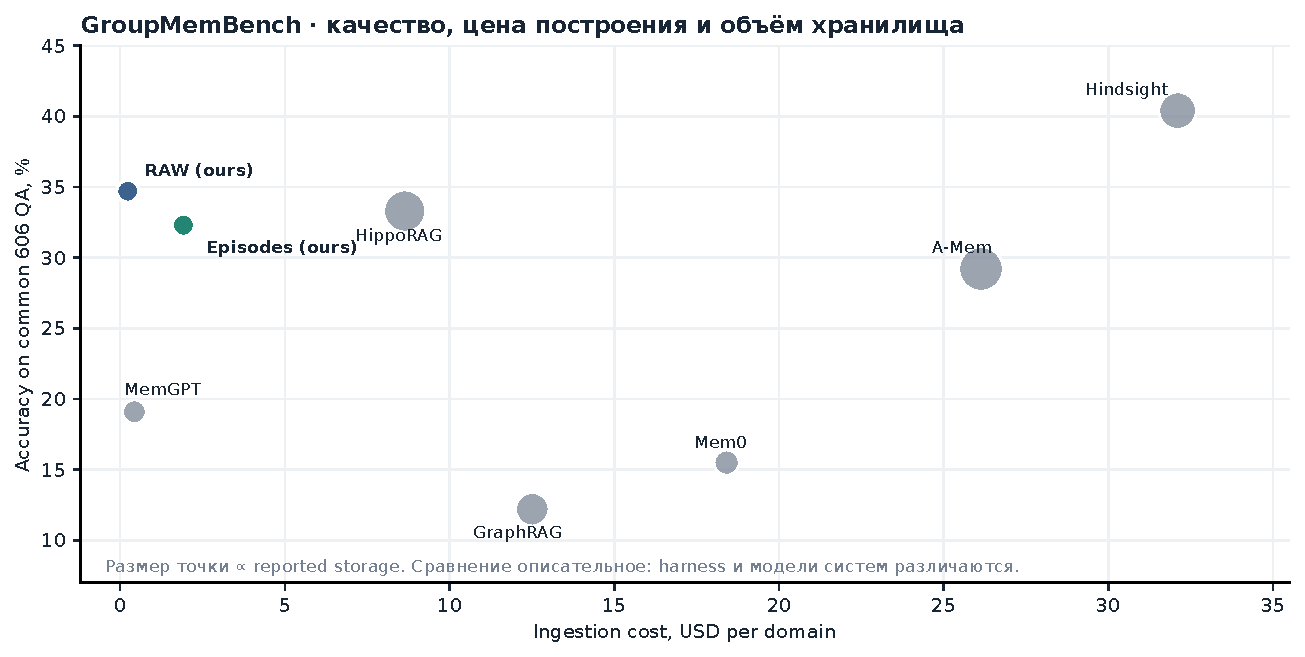
\includegraphics[width=.94\linewidth]{figures/efficiency.pdf}
\caption{Описательный GroupMemBench efficiency landscape на общей выборке
606 QA по значениям benchmark paper и нашего adapter. Размер точки кодирует
reported storage. Наши точки используют repaired amendment; определения
стоимости и backend различаются, поэтому график описывает инженерный trade-off,
а не контролируемое сравнение цены при равном качестве.}
\label{fig:efficiency}
\end{figure}

\begin{table}[ht]
\centering
\small
\begin{tabular}{@{}lrrr@{}}
\toprule
Система & Accuracy, \% & Ingestion, \$/domain & Storage, GB \\
\midrule
Hindsight & 40{,}4 & 32{,}10 & 4{,}25 \\
\textbf{\raw{} (ours)} & \textbf{34{,}7} & \textbf{0{,}23} & \textbf{0{,}37} \\
HippoRAG & 33{,}3 & 8{,}64 & 5{,}76 \\
\textbf{\episodes{} (ours)} & \textbf{32{,}3} & \textbf{1{,}92} & \textbf{0{,}41} \\
A-Mem & 29{,}2 & 26{,}13 & 6{,}60 \\
MemGPT & 19{,}1 & 0{,}43 & 0{,}69 \\
Mem0 & 15{,}5 & 18{,}41 & 0{,}99 \\
GraphRAG & 12{,}2 & 12{,}51 & 3{,}00 \\
\bottomrule
\end{tabular}
\caption{Явные значения для рис.~\ref{fig:efficiency}. Accuracy~--- агрегат по пяти
non-abstention типам задач GroupMemBench (606 QA): для опубликованных систем он
пересчитан из процентов по типам (приложение~\ref{app:group-external}), для наших~---
посчитан по repaired results. Это сопоставление агрегатов, а не единый прогон всех
систем. Ingestion cost и storage взяты из соответствующих benchmark reports. Наши accuracy пересчитаны после targeted repair; стоимость
repair ответов не включена в ingestion. Backend, harness и определения storage
различаются, поэтому сравнение является описательным.}
\label{tab:efficiency}
\end{table}

На этой общей выборке Hindsight достигает 40{,}4\% при reported ingestion
\$32,10/domain и 4,25 GB; HippoRAG~--- 33,3\%, \$8{,}64 и 5{,}76 GB;
наш \raw{}~--- 34{,}7\%, \$0,23 и 0,37 GB; \episodes{}~--- 32,3\%, \$1{,}92 и
0{,}41 GB. Система экономична относительно тяжёлых структурных решений, но
Hindsight точнее. Из-за разных harness-компонентов это контекст, а не
контролируемая причинная оценка цены.

Adapter достигает accuracy на уровне HippoRAG без крупного graph/database
backend: по опубликованным величинам построение Hindsight дороже нашего
\episodes{} примерно в 16{,}7 раза, а storage больше в 10{,}4 раза; для HippoRAG
эти отношения составляют 4{,}5 и 14{,}0. Это отношения reported затрат и объёмов,
а не измерения потребления RAM на одинаковом workload.

\paragraph{Что известно о скорости.}
На 2400 вопросах EverMemBench локальное ранжирование занимает в среднем
11{,}59 мс у RAW и 13{,}70 мс у EPISODES: добавка 2{,}11 мс, около 18\%.
Соответствующие p95~--- 12{,}70 и 15{,}04 мс; сеть и генерация не включены.
Сопоставимого измерения end-to-end query latency чужих memory-систем в
использованных benchmark-таблицах нет, поэтому скорость с другими системами не
сравнивается; длительность полного прогона зависит также от API latency, числа
workers, retries и rate limits.

\subsection{Инженерный смысл}
Построение памяти оплачивается до вопросов; поиск не вызывает linker
повторно. Hot-view ограничивает размер индексируемого эпизода, а cold history
сохраняет все evidence pointers. Поэтому поисковое описание можно исправлять,
не удаляя первичную историю. Запечатывание входов и кэширование позволяют
отделить изменение метода от повторного sampling; спецификация приведена в
приложении.

\section{Риски и возможные ошибки}
\label{sec:errors}

\paragraph{Пропуск extraction.}
Если событие не создано, факт остаётся доступен только через \raw{}.
Structured output ограничивает формат, но не гарантирует полноту извлечения.

\paragraph{Attribution и semantic overreach.}
Буквально существующая цитата может поддерживать только часть описания;
пересказ может принять автора сообщения за владельца мнения. Поэтому 100\%
quote-validity означает целостность адреса, а не 100\% корректных фактов.

\paragraph{False split и false merge.}
Свободные subject/facet формулировки могут раскалывать одну линию на несколько
эпизодов; retrieval может пережить такой split, если обе записи независимо
попадают в контекст. Ошибочное слияние может приносить нерелевантный контекст в
последующие обращения. Консервативные решения resolver могут уменьшать
ошибочные объединения ценой разрыва цепочек; частоты split и merge в работе не
измерялись.

\paragraph{Context displacement.}
Derived hit занимает место в top-$k$ и может вытеснять полезный raw turn. Это
возможное объяснение нейтрального или отрицательного переноса, в частности на
speaker-conditioned GroupMemBench, но не установленная причина: без gold-разметки
источников Group его нельзя проверить напрямую.

\section{Ограничения}
\label{sec:limits}

\paragraph{Два главных пробела.}
Первый: в работе нет сравнения с обычным пересказом тех же сообщений,
снабжённым теми же источниками и полями speaker/time. Поэтому улучшение доставки
установлено для событийного индекса относительно сырого поиска, но не для
событийной схемы относительно более простого derived-представления. Второй:
temporal-выигрыш найден на post hoc выбранном срезе, и все его контроли
используют те же 300 вопросов; независимой проверки на новом наборе нет. Оба требуют
отдельных экспериментов.

\paragraph{Что именно измерено.}
Gold-source delivery не означает достаточность контекста или использование
опоры генератором. Quote-validity проверяет адрес и буквальную цитату, не
entailment derived claim; независимый human-аудит событий не завершён. В
GroupMemBench нет gold source IDs ни в одном из 745 QA, поэтому доставка
источников на нём не измерялась.

\paragraph{Что ещё не разделено.}
Генератор получает и найденные сообщения, и derived-текст. Контроль с
одинаковыми источниками, но без поискового описания подготовлен (B1), однако
завершённых ответов и вердиктов не найдено. Следовательно, вклад выбора
источников пока не отделён от интерпретационной подсказки генератору.

\paragraph{Границы переноса.}
Выводы относятся к данному экстрактору, бюджетам и
bounded conversation spaces; более сильный extractor, веса linking и cap
событий не аблированы. Опубликованные строки других систем, стоимость и storage
сравниваются описательно; они не являются контролируемым production TCO.

\section{Заключение}

Событийная память с адресуемыми источниками разделяет \emph{как искать} и
\emph{чем обосновывать}: самостоятельное описание события делает короткие и
разнесённые реплики доступными semantic retrieval, а неизменяемая provenance
возвращает исходное сообщение с автором и временем.

Главный результат работы~--- улучшение доставки размеченных источников. На
EverMemBench событийный индекс повышает precision gold-источников на
$3{,}21\pp$ и recall на $0{,}64\pp$, возвращая меньше уникальных источников и
больше gold-попаданий; направление сохраняется во всех пяти проектах и
поддерживается на SocialMemBench. На Temporal Duration события сохраняют
преимущество в accuracy (19{,}3\% против 14{,}0\% у RAW и HyDE) после контролей
объёма, порядка и расширения запроса; это exploratory-сигнал, требующий
независимой проверки.

Раздельная оценка доставки и ответа показывает границу установленного: средний
прирост accuracy от событий и добавочный средний прирост от связывания в эпизоды
не установлены, перенос между бенчмарками неоднороден. Для исследуемого
поискового сценария это даёт практический выбор: отдельные \events{}~--- простая
основа поискового слоя, улучшающая доставку источников, а \episodes{}~---
инспектируемая история пересмотров, подтверждений и дополнений. Сильный \raw{}
обеспечивает большую часть общего уровня системы, поэтому новые derived-слои
стоит оценивать парно против него и сразу по двум эндпоинтам~--- доставке
источников и качеству ответа.

\FloatBarrier
\begingroup
\small
\bibliographystyle{plainnat}
\bibliography{references}
\endgroup
\clearpage
\appendix

\section{Полные разрезы EverMemBench}

\begin{table}[ht]
\centering\small
\begin{tabular}{lrrrr}
\toprule
Тип & $n$ & RAW & EVENTS & EPISODES\\
\midrule
Constraint & 402 & 79{,}9 & 79{,}1 & 79{,}6\\
Multi-hop & 249 & 12{,}9 & 13{,}3 & 13{,}3\\
Proactivity & 427 & 65{,}8 & 64{,}6 & 64{,}2\\
Single-hop & 213 & 89{,}7 & 89{,}7 & 87{,}8\\
Skill & 169 & 33{,}7 & 32{,}0 & 30{,}8\\
Style & 176 & 30{,}1 & 33{,}5 & 38{,}1\\
Temporal Duration & 300 & 12{,}3 & 16{,}3 & 20{,}0\\
Title & 196 & 46{,}4 & 45{,}9 & 43{,}4\\
Update & 268 & 46{,}3 & 47{,}0 & 47{,}4\\
\bottomrule
\end{tabular}
\caption{Accuracy по всем официальным категориям, проценты. EVENTS здесь~---
полный experiment A без token/order controls.}
\label{tab:ever-slices}
\end{table}

\section{GroupMemBench: абсолютные результаты по задачам}
\label{app:group-external}

\begin{table}[ht]
\centering\small
\begin{tabular}{@{}lrrrrr@{}}
\toprule
Система & Multi-hop & Update & Ambiguity & Implicit & Temporal\\
\midrule
BM25 & 40{,}11 & 25{,}23 & 14{,}15 & 40{,}82 & 54{,}94\\
Dense RAG & 36{,}26 & 23{,}36 & 21{,}70 & 46{,}94 & 32{,}72\\
Hindsight & 42{,}31 & 17{,}76 & 37{,}74 & 40{,}82 & 54{,}94\\
HippoRAG & 39{,}56 & 27{,}10 & 30{,}19 & 42{,}86 & 29{,}63\\
A-Mem & 35{,}16 & 22{,}43 & 26{,}42 & 46{,}94 & 23{,}46\\
MemGPT & 22{,}53 & 17{,}76 & 20{,}75 & 28{,}57 & 12{,}42\\
Mem0 & 21{,}98 & 4{,}67 & 11{,}32 & 20{,}41 & 16{,}67\\
GraphRAG & 12{,}09 & 14{,}02 & 19{,}81 & 14{,}29 & 5{,}56\\
\midrule
\raw{} (ours, repaired) & 37{,}91 & 28{,}04 & 25{,}47 & 48{,}98 & 37{,}04\\
\episodes{} (ours, repaired) & 34{,}07 & 23{,}36 & 24{,}53 & 48{,}98 & 36{,}42\\
$n$ нашего среза & 182 & 107 & 106 & 49 & 162\\
\bottomrule
\end{tabular}
\caption{GroupMemBench, accuracy в процентах. Внешние строки: таблица 2
arXiv:2605.14498v1 \citep{yang2026}; Dense RAG использует
text-embedding-3-large. Наши строки пересчитаны по repaired results.
Наши знаменатели по пяти типам согласуются с опубликованными процентами;
это не подтверждает побайтное совпадение question files или harness.}
\label{tab:group-external}
\end{table}

Сумма пяти знаменателей равна 606; на этих non-abstention задачах построен
efficiency landscape в основном тексте. Агрегат считается как
$A_{606}=\sum_t n_t a_t\big/\sum_t n_t$, где $a_t$~--- опубликованная accuracy
системы на типе $t$, а $n_t$~--- число вопросов этого типа в наших артефактах
(182, 107, 106, 49 и 162 для Multi-hop, Update, Ambiguity, Implicit и Temporal).
Почти во всех ячейках $n_t a_t$ даёт целое число верных ответов, что согласует
наши знаменатели с опубликованными процентами; у MemGPT на Temporal (12,42\%)
целого числа нет, и количество округлено до ближайшего. Так, для Hindsight
$A_{606}=245/606=40{,}4\%$, для нашего RAW~--- $210/606=34{,}7\%$, для
EPISODES~--- $196/606=32{,}3\%$. Совпадение знаменателей не доказывает
побайтно одинаковый набор вопросов, поэтому это сопоставление non-abstention
агрегатов, а не общий прогон. Значение 40{,}4\% у Hindsight не сопоставимо с
41{,}5\% нашего EPISODES на всех 745 QA: это разные множества вопросов. В опубликованной таблице с abstention средняя accuracy
Hindsight равна 46{,}01\%, BM25~--- 43{,}22\%; у нас на всех 745 QA~---
43{,}09\% RAW и 41{,}48\% EPISODES. Но abstention содержит 139 вопросов
в наших артефактах против 109, согласующихся с опубликованными процентами,
поэтому эти четыре
общие цифры приводятся раздельно, без общего ранжирования.

Таблица показывает, почему одной общей accuracy недостаточно: Hindsight
сильнее на Multi-hop и Ambiguity, наш RAW высок на Update и Implicit,
а BM25 остаётся сильным ориентиром для Temporal. Различие Temporal
GroupMemBench и Temporal Duration EverMemBench также существенно:
первый набор проверяет порядок и относительные выражения времени, второй~--- длительность между границами событий. Межбенчмарковый разрыв процентов
не является сам по себе показателем ухудшения модели.

\section{Доставка свидетельств по категориям}

\begin{center}
\centering\small
\begin{tabular}{lrrr}
\toprule
Тип & $n$ & $\Delta$ precision & 95\% ДИ\\
\midrule
Single-hop & 213 & $+8{,}28$ & $[+6{,}50;+10{,}12]$\\
Temporal Duration & 300 & $+7{,}51$ & $[+5{,}92;+9{,}11]$\\
Style & 176 & $+6{,}31$ & $[+4{,}82;+7{,}84]$\\
Update & 268 & $+3{,}24$ & $[+2{,}12;+4{,}39]$\\
Skill & 169 & $+2{,}32$ & $[+1{,}04;+3{,}73]$\\
Multi-hop & 249 & $+1{,}63$ & $[+0{,}59;+2{,}67]$\\
Title & 196 & $+1{,}55$ & $[+0{,}85;+2{,}30]$\\
Proactivity & 427 & $+1{,}13$ & $[+0{,}77;+1{,}52]$\\
Constraint & 402 & $+0{,}30$ & $[-0{,}07;+0{,}69]$\\
\bottomrule
\end{tabular}
\captionof{table}{\events{}$-$\raw{}, парная разница evidence precision по девяти
официальным категориям EverMemBench, проценты и п.п. Знак положителен везде;
ДИ исключает ноль в восьми категориях из девяти. Сравните с
таблицей~\ref{tab:ever-slices}: категория с наибольшим приростом доставки
(Single-hop) не показывает выигрыша accuracy; её исходный уровень уже 89{,}7\%.}
\label{tab:evid-cats}
\end{center}

\section{Офлайновая редакторская проверка}
\label{app:verification}

Ключевые micro/macro и evidence-агрегаты независимо сверены с пер-вопросными
строками. Для всех 2400 Ever-вопросов gold source IDs восстановлены из
официальных reference spans; пересечения с раскрытыми источниками точно
совпали с сохранёнными precision/recall. Таблица ниже~--- дополнительная
описательная проверка устойчивости направления, выполненная после экспериментов,
не новый зарегистрированный endpoint.

\begin{table}[ht]
\centering\small
\begin{tabular}{lrrr}
\toprule
Проект & $n$ & $\Delta$ precision & $\Delta$ recall\\
\midrule
01 & 488 & $+2{,}50$ & $+0{,}50$\\
02 & 471 & $+3{,}45$ & $+0{,}73$\\
03 & 467 & $+3{,}22$ & $+0{,}51$\\
04 & 481 & $+3{,}61$ & $+0{,}75$\\
05 & 493 & $+3{,}28$ & $+0{,}70$\\
\bottomrule
\end{tabular}
\caption{EVENTS$-$RAW по пяти проектам EverMemBench, п.п.}
\end{table}

При исключении любого одного проекта средний прирост precision составляет
от $3{,}11$ до $3{,}39\pp$ Это чувствительность на данном наборе, не подтверждение
переноса на новые проекты. Social-интервалы в основном тексте дополнительно
пересчитаны network bootstrap: 10\,000 выборок из 43 сетей с возвращением,
пер-вопросная дельта с весом фактического размера сети, seed 20260917.

Распределение числа Ever gold anchors: минимум 4, медиана 27,
межквартильный диапазон 21--37, среднее 30{,}12, максимум 96. Правильный verdict
при нулевом gold intersection наблюдается в 316 RAW, 312 EVENTS и
305 EPISODES ответах. Эти случаи выделяют пределы reference-based метрики,
но не являются самостоятельным аудитом достаточности или верности ответа.

При повторной генерации и оценке одного EPISODES-условия на 300 вопросах
изменились 12 verdicts (по шесть в каждую сторону), а evidence-метрики
совпали во всех вопросах. Равенство относится к фиксированному retrieval
этого контроля, не к произвольной будущей конфигурации.

Дополнительный контроль RAW count-matched возвращает столько сообщений,
сколько раскрывает EPISODES на том же вопросе: accuracy 13{,}3\%, recall 16{,}6\%,
precision 25{,}1\%. Он также не воспроизводит наблюдаемый temporal-уровень
событий. В RAW chrono relative исходные абсолютные временные метки
заменены относительными при том же наборе источников: accuracy 8{,}3\%,
evidence-метрики неизменны. Это отдельный контроль временного оформления,
не контроль удаления derived-текста.

Проверка опубликована в исходниках статьи как
\path{verify_editorial.py}; её отчёт \path{editorial_verification.json}
содержит hashes прочитанных входов. Артефакты экспериментов не изменяются.
Экстремальные Wilcoxon $p$ прежнего черновика исключены: старый helper
не усреднял ранги при совпадениях; размеры эффектов и bootstrap-интервалы
от этого helper не зависят.

\section{Точность выравнивания токен-бюджета}
\label{app:tokens}

Сопоставлены сохранённые \texttt{context\_tokens} по одинаковым 300 QA keys,
без восстановления промптов или новых генераций. Счётчик использует
\texttt{o200k\_base}; учитывается раскрытый контекст с оформлением блоков,
но без вопроса и общей инструкционной рамки. Для пары условий $a,b$
отклонение равно $|T_a(q)-T_b(q)|$, относительное~---
$100|T_a(q)-T_b(q)|/T_b(q)$. Процентили считаются отдельно для абсолютных
и относительных отклонений: процент в таблице не является отношением
двух отдельно усреднённых величин.

\begin{table}[ht]
\centering\small
\begin{tabular}{lrrrr}
\toprule
Пара chrono-контекстов & Медиана & 95-й перц. & Максимум & Медиана, \%\\
\midrule
RAW~--- EPISODES & 25 & 56{,}1 & 83 & 0{,}99\\
EVENTS~--- EPISODES & 26 & 73{,}1 & 137 & 1{,}08\\
HyDE~--- EVENTS & 25 & 55{,}1 & 97 & 1{,}06\\
EVENTS~--- RAW & 35 & 97{,}0 & 139 & 1{,}48\\
\bottomrule
\end{tabular}
\caption{Абсолютные пер-вопросные отклонения token matching, в токенах,
кроме последнего столбца. Знаменатель относительного отклонения~---
второе условие пары; все контексты упорядочены хронологически.}
\end{table}

Для ключевого сравнения EVENTS~--- RAW межквартильный диапазон абсолютной
разницы составляет 16--58 токенов; 95-й перцентиль относительной разницы
4{,}60\%, максимум 11{,}46\%. Для EVENTS~--- HyDE соответствующие медиана,
95-й перцентиль и максимум равны 25, 55{,}1 и 97 токенам; относительные
значения~--- 1{,}06\%, 3{,}22\% и 8{,}76\%. Средние контексты RAW, EVENTS,
HyDE и EPISODES составляют 2458{,}1; 2456{,}1; 2451{,}4 и 2459{,}7 токена.
Matching сближает бюджеты, но не устраняет различие размера на каждом
вопросе. Эти отклонения не являются отдельной абляцией остаточного объёма.
Расчёт включён в \path{verify_editorial.py} и
\path{editorial_verification.json}, раздел \texttt{token\_matching}.

\section{Связь evidence и accuracy: протокол анализа}
\label{app:frontier}

Протокол \path{research/FRONTIER_MECHANISM_PREDICTION_PROTOCOL.md}
фиксирует до расчёта этого анализа три страты вне Temporal Duration:
A~--- EVENTS не хуже по recall и precision и строго лучше хотя бы по одной
координате; B~--- аналогично доминирует RAW; C~--- смешанный результат
или равенство. Правило подтверждения требует положительной значимой
accuracy-дельты в A, отрицательного направления в B и интервала,
содержащего ноль, в C. Основное условие A не выполнено. Небольшое число
discordant пар (77, 23, 67) ограничивает мощность; ДИ допускают и полезный
положительный эффект. Анализ не устанавливает причинный bottleneck.

\begin{table}[ht]
\centering\small
\begin{tabular}{lrrrrr}
\toprule
Страта & $n$ & $\Delta$acc & 95\% ДИ & выигр./проигр. & McNemar\\
\midrule
A (события доминируют) & 650 & $+0{,}77$ & $[-1{,}85;+3{,}54]$ & 41/36 & $.649$\\
B (\raw{} доминирует) & 209 & $-2{,}39$ & $[-6{,}70;+2{,}39]$ & 9/14 & $.405$\\
C (смешанный) & 1241 & $-0{,}24$ & $[-1{,}53;+1{,}05]$ & 32/35 & $.807$\\
\bottomrule
\end{tabular}
\caption{Офлайновая проверка связи доставки и ответа на 2100 вопросах вне discovery-среза,
\events{}$-$\raw{}, проценты и п.п.}
\label{tab:frontier}
\end{table}

\section{GroupMemBench: восстановление пустых ответов}
\label{app:repair}

Исходный прогон имел 102 пустых ответа из 1490: 44 RAW и 58 EPISODES.
Amendment повторяет только эти вызовы с теми же sealed prompts и повышенным
output budget; все 102 восстановлены. Остальные 1388 ответов сохранены
побайтно, source IDs неизменны. Исходные результаты не переписаны.

\begin{table}[ht]
\centering\small
\begin{tabular}{llrrrr}
\toprule
Срез & Версия & $n$ & RAW & EPISODES & $\Delta$ [95\% ДИ]\\
\midrule
Primary & исходная & 150 & 34{,}0 & 30{,}0 & $-4{,}0\ [-9{,}3;1{,}3]$\\
Primary & repair & 150 & 37{,}3 & 33{,}3 & $-4{,}0\ [-9{,}3;1{,}3]$\\
Все QA & исходная & 745 & 42{,}0 & 40{,}3 & $-1{,}7\ [-4{,}3;0{,}7]$\\
Все QA & repair & 745 & 43{,}1 & 41{,}5 & $-1{,}6\ [-4{,}0;0{,}8]$\\
\bottomrule
\end{tabular}
\caption{GroupMemBench до и после repair, проценты и п.п.
Primary: Finance+Technology, knowledge update+temporal.}
\end{table}

Repair стоил \$2,69; около 94\% output tokens пришлись на hidden reasoning.
Один общий payload был вызван дважды при параллельном заполнении cache;
финальные ответы совпали. Repair является post-protocol amendment,
не официальной leaderboard submission.

Проверены все 745 официальных QA: каждый содержит идентификатор вопроса,
его текст, эталонный ответ и идентификатор спрашивающего участника.
Ни source IDs, ни evidence spans в этой версии questions нет.
Нельзя объявить evidence recall/precision, восстановив gold из самого
ответа без отдельной разметки. Гипотеза вытеснения полезных источников
на Group остаётся непроверенной. Раскрытые IDs обоих условий сопоставимы
и найдены в корпусе из 120\,000 сообщений; недостаёт именно gold-множества.

\section{Воспроизведение: модели, промпты и масштаб памяти}
\label{app:reproduce}

\begin{table}[ht]
\centering\small
\begin{tabular}{@{}lrrr@{}}
\toprule
 & EverMemBench & SocialMemBench & GroupMemBench\\
\midrule
Сети / проекты & 5 & 43 & 4\\
Сессии извлечения & 3570 & 348 & 3153\\
Сообщения & 51\,023 & 7355 & 120\,000\\
События после валидатора & 16\,859 & 639 & 21\,407\\
Отклонено валидатором & 4548 & 428 & 6822\\
Эпизоды & 9298 & 449 & 10\,801\\
Решения attach: NEW & 9298 & 449 & 10\,801\\
\quad AUGMENT & 5175 & 151 & 5586\\
\quad REAFFIRM & 1482 & 11 & 2331\\
\quad REVISE & 904 & 28 & 2689\\
\bottomrule
\end{tabular}
\caption{Масштаб построенной памяти. Каждое сохранённое событие получает ровно одно
решение attach, поэтому сумма решений равна числу событий, а число NEW~--- числу
эпизодов. Счётчики взяты из запечатанных \texttt{episodes\_meta.json} и
\texttt{attach\_decisions.jsonl}.}
\label{tab:memory-scale}
\end{table}

\begin{sloppypar}
\paragraph{Модели и настройки памяти.}
Извлечение событий и решения attach выполняет \texttt{gpt-4o-mini-2024-07-18}
при \texttt{temperature}${}=0$, \texttt{max\_tokens}${}=8192$ и JSON-выводе. Сессия
передаётся целиком, по строке на сообщение:
\texttt{[[turn\_id]] [ANCHOR] время говорящий: текст}. На одно сообщение~--- не более
двух событий. Кандидаты для attach~--- три лучших эпизода по скору $S(e,E)$ на
локальных эмбеддингах \texttt{paraphrase-multilingual-MiniLM-L12-v2}; при confidence
ниже 0,5 создаётся новый эпизод; hot view~--- пять последних событий. Retrieval
ответов: \texttt{text-embedding-3-large} (EverMemBench, GroupMemBench) и
\texttt{text-embedding-3-small} (SocialMemBench), cosine top-10.

\paragraph{Шаблоны документов.}
Индексный текст события: \texttt{Viewpoint owner: <o>. Subject: <s>. <z>}; у эпизода
вместо $z$ стоят тексты пяти последних событий через \texttt{||}. Генератор получает
заголовок \texttt{[DERIVED EVENT / owner=<o> / subject=<s>]}, текст события и по строке
\texttt{[SOURCE <id>]} на каждый источник из $P$; сообщения из $L$ в этот документ не
входят.

\paragraph{Где промпты и как пересчитать.}
Промпт извлечения и промпт attach~--- функции \path{_event_extraction_prompt} и
\path{_attach_prompt} в \path{reproduction/research/temporal_episode_prototype.py};
adapters бенчмарков лежат рядом. Все числа статьи пересчитываются офлайн, без
ключей API:
\begin{quote}\small
\texttt{python3 analysis/verify\_results.py}\\
\texttt{python3 analysis/verify\_evidence\_endpoint.py}
\end{quote}
Повторные прогоны требуют ключей OpenAI и OpenRouter; команды по бенчмаркам
перечислены в \path{REPRODUCE.md}, например
\texttt{python3 -m research.evermembench\_parallel\_resume --all}.
\end{sloppypar}

\section{Точная спецификация хранения}

\begin{table}[ht]
\centering\small
\begin{tabularx}{\linewidth}{lX}
\toprule
Единица & Поля и назначение\\
\midrule
RawTurn & ID, conversation network, speaker, timestamp, text; неизменяемый адрес.\\
MemoryEvent & ID, index text, type, viewpoint owner, subject, temporal mode,
observed time, evidence, local context.\\
EventEvidence & Event ID, raw source ID, literal quote; проверяемая связь.\\
EpisodeEvent & Episode ID, Event ID, order, attach operation; append-only история.\\
SearchDocument & kind, index text, render text, source IDs; общий retrieval interface.\\
\bottomrule
\end{tabularx}
\caption{Логическая схема не зависит от JSONL, SQLite или PostgreSQL backend.}
\end{table}

\section{Артефакты и границы утверждений}

Код, протоколы и конфигурации:
\url{https://github.com/yaroslavlikh/temporal-episodes} (репозиторий закрыт до
публикации). Что именно он распространяет, определяется лицензией каждого
бенчмарка: пер-вопросные предсказания и вердикты для EverMemBench (данные под
Apache 2.0) и SocialMemBench (CC BY 4.0), а для GroupMemBench, у которого
лицензии нет,~--- только агрегаты и SHA-256 удержанных пер-вопросных файлов.
Кэши моделей, эмбеддинги и сами корпуса не распространяются. Идентификаторы и
хэши запечатанных прогонов перечислены ниже.

Основные immutable каталоги:
\begin{itemize}
\item \texttt{evermembench\_temporal\_episodes\_official\_v1\_20260915\_021550\_MSK};
\item \texttt{final\_sprint\_A\_events\_full\_v1\_20260915\_233142\_MSK};
\item \texttt{final\_sprint\_B2\_episodes\_chrono\_v1\_20260915\_232910\_MSK};
\item \texttt{final\_sprint\_C\_hyde\_raw\_v1\_20260916\_024144\_MSK};
\item \texttt{final\_sprint\_C2\_hyde\_token\_matched\_v1\_20260916\_024306\_MSK};
\item \texttt{socialmembench\_temporal\_episodes\_official\_harness\_v1\_20260912\_122626\_MSK}.
\end{itemize}
Дополнительный sealed amendment GroupMemBench хранится в
\path{final_sprint_D_groupmembench_repair_v2} (1490 строк), SHA-256:
\begin{center}\small
\begin{tabular}{@{}ll@{}}
\texttt{results\_v2} & \texttt{41ae844eabb292f9d0c7edbeed0476981155340ac85c5ef197d2184fcbd0d4a5}\\
\texttt{predictions\_v2} & \texttt{20f2c60180a58d37c63f96904896266c8ac5805f83d822d321a34926850c8a96}
\end{tabular}
\end{center}
Каталог не копировался в отдельный frozen container; восемь исходных файлов
проверены по manifest и не изменены.
Использованные revisions: EverMemBench code \texttt{e10b3d52f0e4}, data
\texttt{a6b210a32248}; GroupMemBench \texttt{e2682e01ff49}. Скрипт фигур
хэширует входные summaries/reports. Публичное размещение кода не означает
автоматического разрешения на перераспространение benchmark corpora.

\paragraph{Какой Social-прогон канонический.}
В артефактах присутствуют два SocialMemBench-пайплайна, и смешивать их нельзя.
Канонический~--- \texttt{socialmembench\_temporal\_}\allowbreak
\texttt{episodes\_official\_harness\_v1}:
\texttt{text-embedding-3-small}, единый cosine top-10 и общий
answer/judge/packing; из него взяты все числа работы, а строки
RAW/FLAT/VERSIONED в нём~--- неизменённые результаты замороженного прогона
2026-09-11. Второй, \path{socialmembench_temporal_episodes_full_v1},~--- более
ранний гибрид (локальная \texttt{MiniLM}, raw top-12 + episode top-12, бюджет
400 слов); его \raw{} даёт evidence recall 48,5\% против 67,5\% у канонического.
Парное сравнение условия из одного прогона с \raw{} из другого даёт
правдоподобные и полностью ложные числа; мы отмечаем это здесь, потому что оба
каталога распространяются вместе.

\paragraph{Входы и воспроизведение.}
Сохранённые evidence effect sizes и question-bootstrap интервалы доступны
в \path{research/figures/evidence_endpoint_results.json}. Скрипт
\path{build_dissociation_figure.py} строит категориальный рисунок по этим
значениям; \path{build_figures.py} фиксирует hashes остальных входов.
Редакторская проверка использует отдельный отчёт и не переписывает результаты.

\end{document}
